

\documentclass[oneside,20pt]{article}          % please do not change
\usepackage[b5paper]{geometry}	    % your paper can be easily printed on a4 or letter paper with enlargenment      
                                    % comment if you have problem with print     
\usepackage{amsfonts,amsmath,latexsym,amssymb}
\usepackage{graphicx}
%%% remove comment delimiter ('%') and specify parameters if required
%\usepackage[dvips]{graphics}

\begin{document}

%%% remove comment delimiter ('%') and select language if required
%\selectlanguage{spanish} 

\noindent 
\begin{center}
  \texttt{LABORATOR 2-- Buffer Overflow în Python, Python Debugger .}        
\end{center}

\section{Buffer Overflow în Python}
\noindent                 
\\\\\
\textbf{Rezumat:}\\
Buffer overflow are loc atunci când datele sunt introduse sau scrise dincolo de limitele alocate unui obiect, provocând o blocare a programului sau creând o vulnerabilitate pe care atacatorii o pot exploata.\\

\textbf{Descriere:}\\
O depășire a memoriei tampon are loc atunci când datele sunt scrise dincolo de limitele unui tampon cu lungime fixă ​​suprascriind locații de memorie adiacente care pot include alte buffere, variabile și date de flux de program. Considerată „bomba nucleară” a industriei software, buffer overflow este una dintre cele mai persistente vulnerabilități de securitate și atacuri frecvent utilizate.  

Risc: Cum se poate întâmpla?
Scrierea în afara limitelor unui bloc de memorie alocată poate deteriora datele, poate bloca programul sau poate provoca execuția de cod rău intenționat. Python, ca și Java, face un efort pentru a evita depășirea buffer-ului verificând limitele unui buffer (precum o matrice) și împiedicând orice acces dincolo de aceste limite. Totuși, niciun limbaj nu este perfect, așa că este esențial ca toți programatorii să înțeleagă conceptele descrise mai jos.

Exemplu real:
Vulnerabilitățile de depășire a unui buffer au fost exploatate de primul atac major pe Internet. Cunoscut sub numele de viermele Morris, acest atac a infectat peste 60.000 de calculatoare și a închis o mare parte a internetului timp de câteva zile în 1988.
Carolyn Duffy Marsan. Morris Worm a fost un atac petrecut în urmă cu câțiva ani buni. Uite ce s-a întâmplat în 30 octombrie 2008:\\ 
https://www.hypr.com/security-encyclopedia/morris-worm\\

Exemplu în cod:\\
Deși Python permite diferite moduri de a crea și de a manipula matrice, dacă utilizați matrice de o dimensiune predeterminată, puteți determina programul să provoace IndexError pentru a evita o depășire a bufferului.\\

\begin{center}
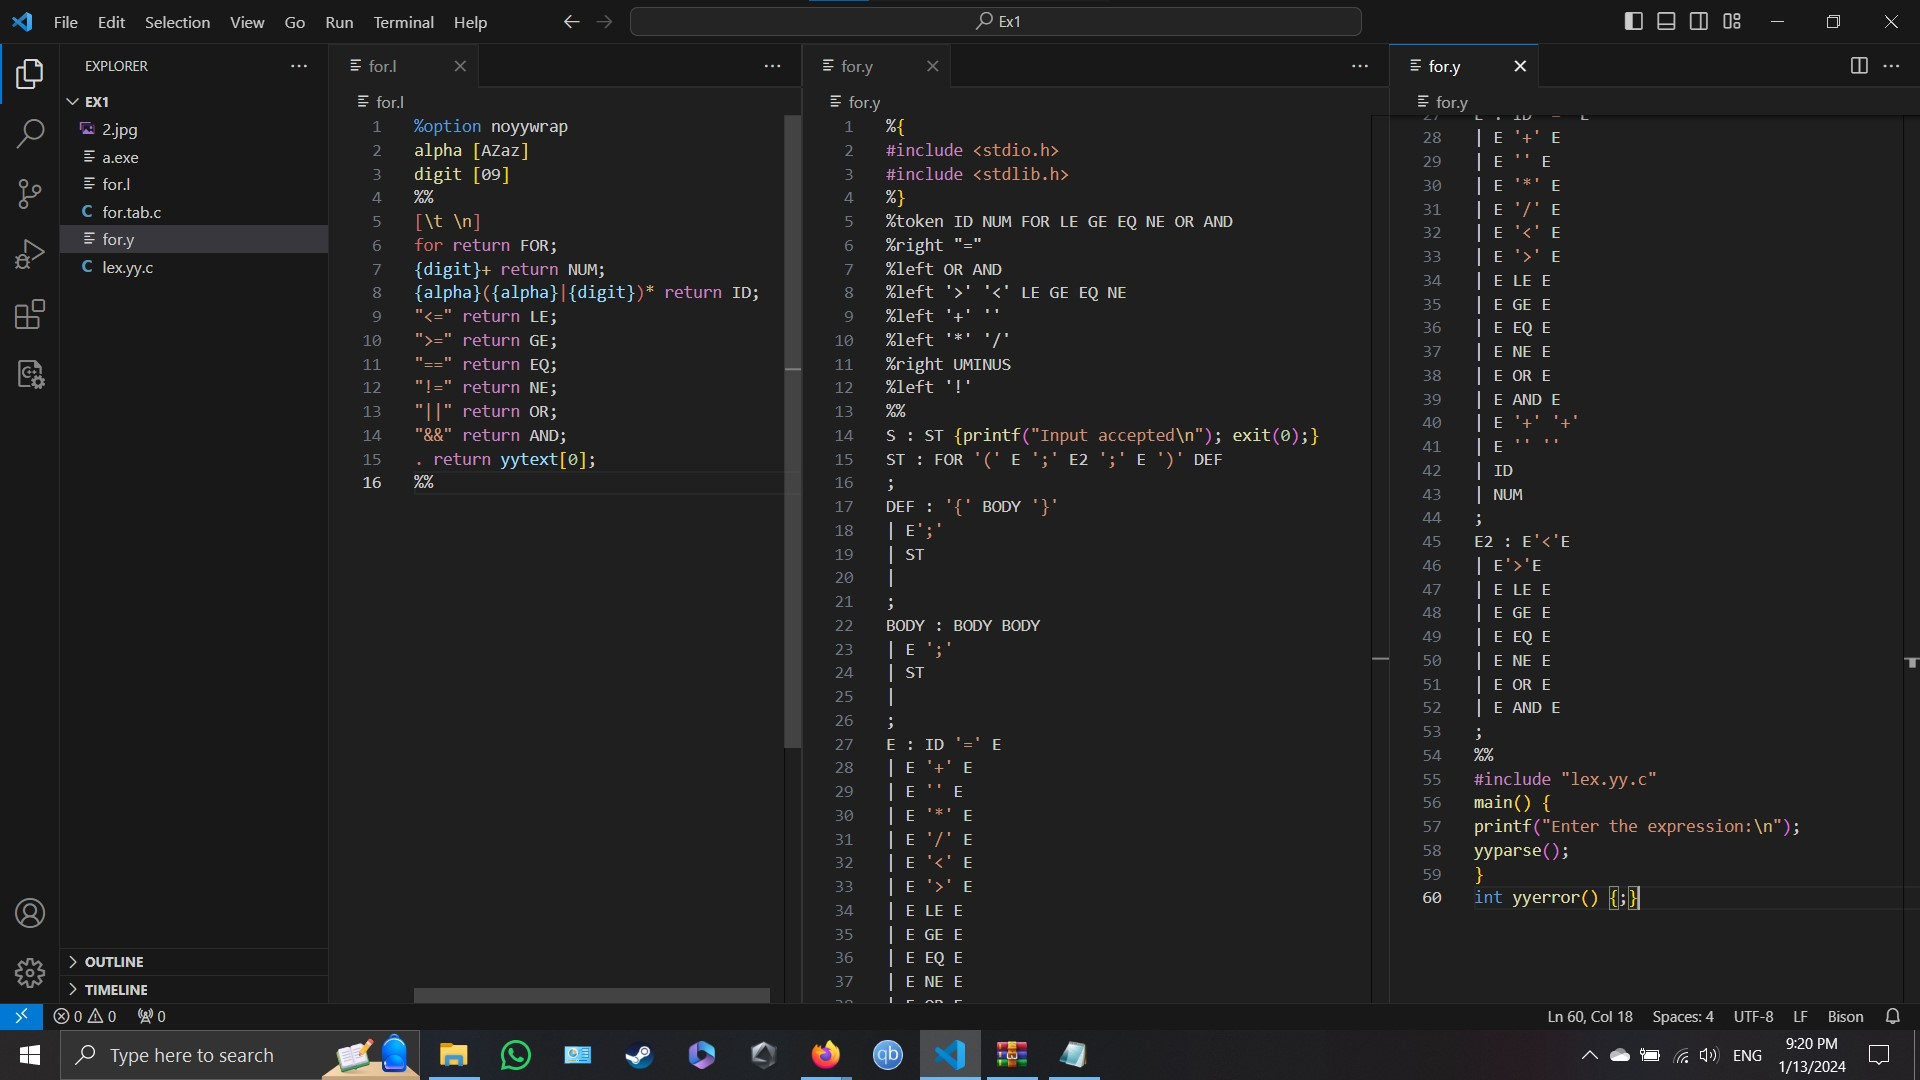
\includegraphics[height = 2 cm]{1.png}
\end{center}
 
În codul de mai sus, bufferul are 10 elemente, dar bucla încearcă să scrie prin 15 elemente, ceea ce duce la o eroare.

Cod responsabil – Cum pot evita depășirea tamponului?

Asigurați-vă că aveți suficient spațiu: înainte de a copia datele într-un bloc de dimensiune fixă, asigurați-vă că este suficient de mare pentru a stoca datele pe care urmează să le copiați. Dacă nu este suficient de mare, nu copiați mai multe date decât poate stoca spațiul disponibil. Dacă programul dvs. nu poate continua corect după ce ați umplut spațiul disponibil, este posibil să fiți nevoit să găsiți o modalitate de a vă recupera din eroare.

Validați indici: dacă aveți o variabilă întreagă, verificați dacă se află în limitele adecvate înainte de a o utiliza ca index pentru o matrice. Această validare este deosebit de importantă pentru orice valoare care ar fi putut fi furnizată ca intrare de utilizator sau alte intrări nesigure, cum ar fi informații care ar putea fi citite dintr-un fișier sau dintr-o conexiune de rețea.

Utilizați structuri de date alternative care reduc riscul de depășire: atunci când este posibil, utilizați liste în Python fără a defini dimensiunea inițială și utilizați metoda .append pentru a adăuga elemente care vă pot reduce riscul de vulnerabilități de depășire a tamponului.
\begin{center}
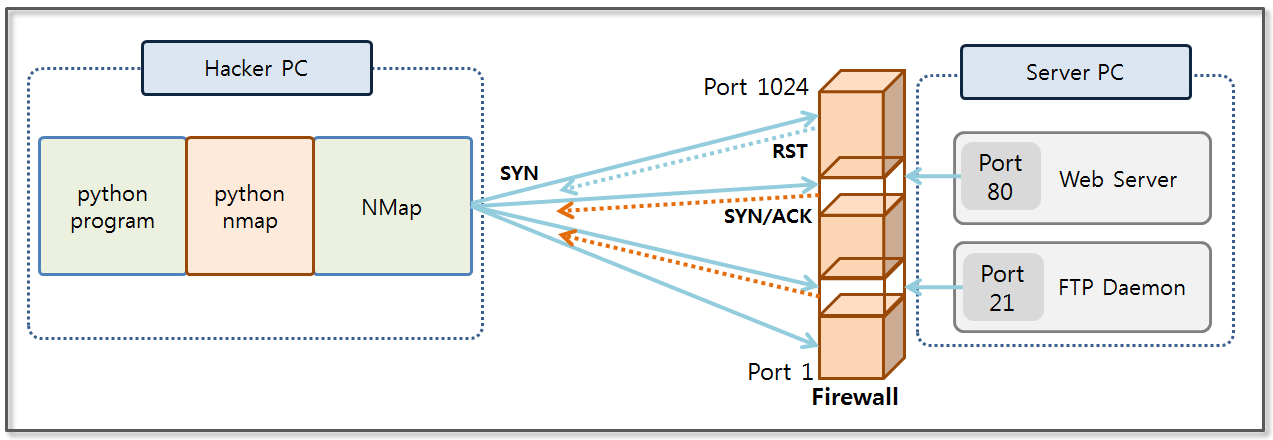
\includegraphics[height = 2 cm]{2.png}
\end{center}
\textbf{Întrebări}:\\
Descrieți problema depășirii buffer-ului.\\\
Cum ați putea preveni o depășire a bufferului să apară în programul dvs.?\\
Lucru suplimentar:\\
Dați trei exemple din viața reală de atacuri de buffer overflow (cercetare pe web).\\
Ce poate rezulta dintr-o depășire a bufferului?\\
Furnizați trei exemple diferite de cod care conține depășiri de buffer.\\
\section{Python Debugger}
\subsection{Clasa pdb}
Modulul pdb definește un depanator interactiv de cod sursă pentru programele Python. Acceptă setarea punctelor de întrerupere (condiționale) și un singur pas la nivelul liniei sursă, inspecția cadrelor stivei, listarea codului sursă și evaluarea codului Python arbitrar în contextul oricărui cadru stivă. De asemenea, acceptă depanarea post-mortem și poate fi apelat sub controlul programului.

Utilizarea tipică pentru a rula un program sub controlul debugger-ului este:
\begin{center}
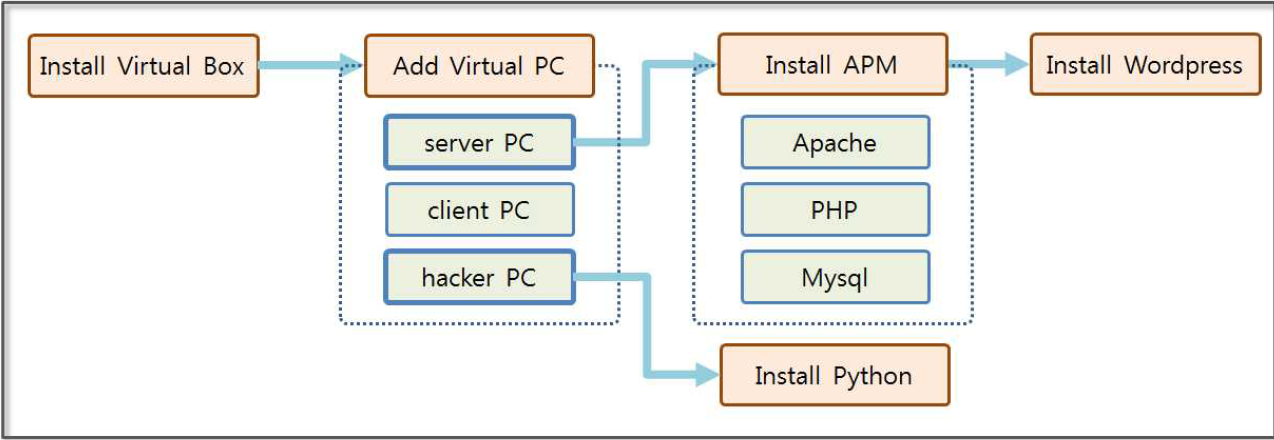
\includegraphics[height = 2 cm]{3.png}
\end{center}
Utilizarea tipică pentru inspectarea unui program blocat este:
\begin{center}
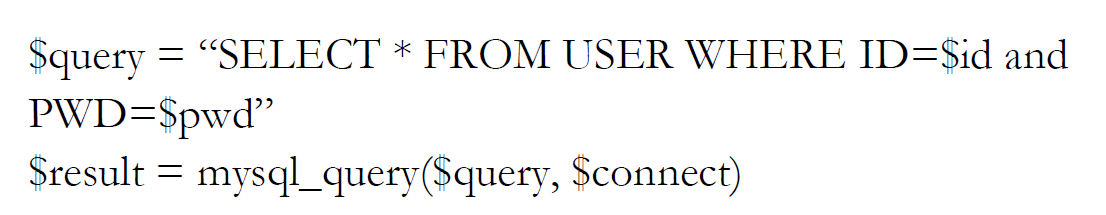
\includegraphics[height = 2 cm]{4.png}
\end{center}
Modulul debugger definește următoarele funcții:
\textbf{
pdb.run(statement, globals=None, locals=None)}\\
Executați instrucțiunea (dată ca șir sau obiect cod) sub controlul debugger-ului. Promptul de depanare apare înainte ca orice cod să fie executat; puteți seta puncte de întrerupere și tastați continue sau puteți parcurge instrucțiunea folosind step sau next (toate aceste comenzi sunt explicate mai jos). Argumentele opționale globale și locale specifică mediul în care este executat codul; implicit este folosit dicționarul modulului main. (Vezi explicația funcțiilor încorporate exec() sau eval().)\\

\textbf{pdb.runeval(expression, globals=None, locals=None)}\\
Evaluați expresia (dată ca șir sau obiect de cod) sub controlul depanatorului. Când runeval() revine, returnează valoarea expresiei. În caz contrar, această funcție este similară cu run().\\
\textbf{
pdb.runcall(function, *args, **kwds)}\\
Apelați funcția (o funcție sau un obiect de metodă, nu un șir) cu argumentele date. Când runcall() revine, returnează orice apelul funcției returnat. Promptul de depanare apare imediat ce funcția este introdusă.\\
\textbf{pdb.set trace(*, header=None)}\\
Introduceți debugger-ul în cadrul stivei de apelare. Acest lucru este util pentru a codifica un punct de întrerupere într-un anumit punct al unui program, chiar dacă codul nu este altfel depanat (de exemplu, când o afirmație eșuează). Dacă este dat, antetul este imprimat pe consolă chiar înainte de a începe depanarea.\\


\textbf{pdb.post mortem(traceback=None)}\\
Introduceți depanarea post-mortem a obiectului de urmărire dat. Dacă nu se oferă nicio urmărire, se utilizează pe cea a excepției care este gestionată în prezent (o excepție trebuie să fie tratată dacă urmează să fie utilizată implicit).\\
\textbf{
pdb.pm()}
Introduceți depanarea post-mortem a urmăririi găsite în sys.last traceback.\\

Funcțiile run* și set trace() sunt alias-uri pentru instanțiarea clasei Pdb și apelarea metodei cu același nume. Dacă doriți să accesați funcții suplimentare, trebuie să faceți acest lucru singur:\\

clasa pdb.Pdb(completekey='tab', stdin=None, stdout=None, skip=None, nosigint=False, readrc=True)\\
Pdb este clasa de depanare.\\

Argumentele completekey, stdin și stdout sunt transmise clasei de bază cmd.Cmd; vezi descrierea acolo.

Argumentul skip, dacă este dat, trebuie să fie un iterabil de modele de nume de modul în stil glob. Depanatorul nu va păși în cadre care provin dintr-un modul care se potrivește cu unul dintre aceste modele. 

În mod implicit, Pdb setează un handler pentru semnalul SIGINT (care este trimis atunci când utilizatorul apasă Ctrl-C pe consolă) atunci când dați o comandă de continuare. Acest lucru vă permite să intrați din nou în depanator apăsând Ctrl-C. Dacă doriți ca Pdb să nu atingă handlerul SIGINT, setați nosigint la true.

Argumentul readrc este implicit adevărat și controlează dacă Pdb va încărca fișiere .pdbrc din sistemul de fișiere.

Exemplu de apel pentru a activa urmărirea cu skip:
\begin{center}
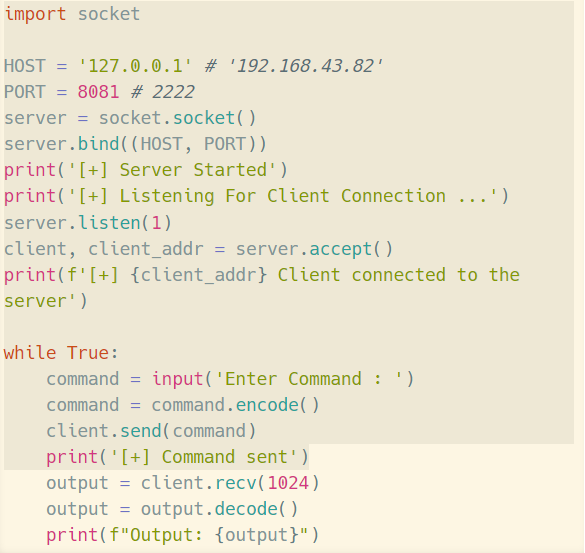
\includegraphics[height = 1 cm]{5.png}
\end{center}
Comenzi de depanare
Comenzile recunoscute de debugger sunt enumerate mai jos. Majoritatea comenzilor pot fi abreviate la una sau două litere, după cum este indicat; de exemplu. h(elp) înseamnă că fie h, fie help pot fi folosite pentru a introduce comanda de ajutor (dar nu he sau hel, nici H sau Help sau HELP). Argumentele la comenzi trebuie separate prin spații albe (spații sau file). Argumentele opționale sunt incluse între paranteze drepte ([]) în sintaxa comenzii; parantezele pătrate nu trebuie dactilografiate. Alternativele din sintaxa comenzii sunt separate printr-o bară verticală (|).

Introducerea unei linii goale repetă ultima comandă introdusă. Excepție: dacă ultima comandă a fost o comandă listă, sunt listate următoarele 11 linii.

Comenzile pe care depanatorul nu le recunoaște sunt presupuse a fi instrucțiuni Python și sunt executate în contextul programului care este depanat. Declarațiile Python pot fi, de asemenea, prefixate cu un semn de exclamare (!). Aceasta este o modalitate puternică de a inspecta programul depanat; este chiar posibil să schimbi o variabilă sau să apelezi o funcție. Când apare o excepție într-o astfel de declarație, numele excepției este tipărit, dar starea depanatorului nu este schimbată.

Debugger-ul acceptă aliasuri. Aliasurile pot avea parametri care permit un anumit nivel de adaptabilitate la contextul examinat.

Pot fi introduse mai multe comenzi pe o singură linie, separate prin ;;. (Un singur ; nu este folosit deoarece este separatorul pentru mai multe comenzi dintr-o linie care este transmisă parserului Python.) Nu se aplică inteligență pentru separarea comenzilor; intrarea este împărțită la prima ;; pereche, chiar dacă se află în mijlocul unui șir între ghilimele. O soluție pentru șiruri de caractere cu punct și virgulă dublu este să utilizați concatenarea implicită a șirurilor de caractere ';'';' sau ";"";".

Dacă un fișier .pdbrc există în directorul principal al utilizatorului sau în directorul curent, acesta este citit cu codificare „utf-8” și executat ca și cum ar fi fost tastat la promptul depanatorului. Acest lucru este util în special pentru aliasuri. Dacă ambele fișiere există, cel din directorul principal este citit primul și aliasurile definite acolo pot fi suprascrise de fișierul local.\\

Modificat în versiunea 3.11: .pdbrc este acum citit cu codificare „utf-8”. Anterior, a fost citit cu codificarea locală a sistemului.\\

Modificat în versiunea 3.2: .pdbrc poate conține acum comenzi care continuă depanarea, cum ar fi continue sau next. Anterior, aceste comenzi nu aveau niciun efect.\\

\textbf{h(elp) [command]}\\
Fără argument, tipăriți lista comenzilor disponibile. Cu o comandă ca argument, imprimați help despre acea comandă. help pdb afișează documentația completă (docstring-ul modulului pdb). Deoarece argumentul comenzii trebuie să fie un identificator, trebuie introdus help exec pentru a obține ajutor pentru ! comanda.

\textbf{w(here) [command]}\\
Imprimați o urmă de stivă, cu cel mai recent cadru în partea de jos. O săgeată indică cadrul curent, care determină contextul majorității comenzilor.\\

\textbf{d(own) [count]}\\
Mutați numărul curent de cadre (unul implicit) în jos în urma stivei (la un cadru mai nou).\\

\textbf{u(p) [count]}\\
Mutați numărul curent de cadre (unul implicit) în sus în urma stivei (la un cadru mai vechi).\\

\textbf{b(reak) [[([nume fișier:]lineno | funcție) [, condiție]]}\\
Cu un argument lineno, setați o pauză acolo în fișierul curent. Cu un argument de funcție, setați o pauză la prima instrucțiune executabilă din acea funcție. Numărul de linie poate fi prefixat cu un nume de fișier și două puncte, pentru a specifica un punct de întrerupere într-un alt fișier (probabil unul care nu a fost încărcat încă). Fișierul este căutat pe sys.path. Rețineți că fiecărui punct de întrerupere i se atribuie un număr la care se referă toate celelalte comenzi ale punctului de întrerupere.\\

Dacă este prezent un al doilea argument, este o expresie care trebuie evaluată la adevărat înainte ca punctul de întrerupere să fie respectat.\\

Fără argument, enumerați toate pauzele, inclusiv pentru fiecare punct de întrerupere, de câte ori acel punct de întrerupere a fost atins, numărul curent de ignorare și condiția asociată, dacă este cazul.\\

\textbf{tbreak [[([nume fișier:]lineno | funcție) [, condiție]]}\\
Punct de întrerupere temporară, care este eliminat automat la prima atingere. Argumentele sunt aceleași ca pentru pauză.\\

\textbf{cl(ear) [nume fișier:lineno | bpnumber ...]}
Cu un argument filename:lineno, ștergeți toate punctele de întrerupere de la această linie. Cu o listă de numere de puncte de întrerupere separate prin spații, ștergeți acele puncte de întrerupere. Fără argumente, ștergeți toate pauzele (dar mai întâi cereți confirmarea).\\
\textbf{
disable [bpnumber ...]}\\
Dezactivați punctele de întrerupere date ca o listă de numere de puncte de întrerupere separate prin spații. Dezactivarea unui punct de întrerupere înseamnă că nu poate determina programul să oprească execuția, dar, spre deosebire de ștergerea unui punct de întrerupere, acesta rămâne în lista punctelor de întrerupere și poate fi (re)activat.\\

\textbf{
enable [bpnumber ...]}\\
Activați punctele de întrerupere specificate.\\

\textbf{ignore bpnumber [count]}\\
Setați numărul de ignorare pentru numărul punctului de întrerupere dat. Dacă numărul este omis, numărul de ignorare este setat la 0. Un punct de întrerupere devine activ când numărul de ignorare este zero. Când nu este zero, numărul este decrementat de fiecare dată când punctul de întrerupere este atins și punctul de întrerupere nu este dezactivat și orice condiție asociată este evaluată la adevărată.\\

\textbf{condition bpnumber [condition]}\\
Setați o nouă condiție pentru punctul de întrerupere, o expresie care trebuie evaluată la adevărat înainte ca punctul de întrerupere să fie respectat. Dacă condiția este absentă, orice condiție existentă este eliminată; adică punctul de întrerupere este făcut necondiționat.\\

\textbf{commands [bpnumber]}\\
Specificați o listă de comenzi pentru numărul punctului de întrerupere bpnumber. Comenzile în sine apar în rândurile următoare. Tastați o linie care conține doar sfârșit pentru a termina comenzile.\\

Pentru a elimina toate comenzile dintr-un punct de întrerupere, tastați comenzi și urmați-le imediat cu sfârșit; adică să nu dai comenzi.\\

Fără argument bpnumber, comenzile se referă la ultimul set de puncte de întrerupere.\\

Puteți utiliza comenzile punct de întrerupere pentru a reporni programul. Pur și simplu utilizați comanda continue, sau pasul sau orice altă comandă care reia execuția.\\

Specificarea oricărei comenzi care reia execuția (continuare în prezent, pas, următor, întoarcere, salt, ieșire și abrevierile acestora) încheie lista de comenzi (ca și cum acea comandă ar fi urmată imediat de sfârșit). Acest lucru se datorează faptului că de fiecare dată când reluați execuția (chiar și cu un simplu următor sau pas), puteți întâlni un alt punct de întrerupere – care ar putea avea propria listă de comenzi, ceea ce duce la ambiguități cu privire la lista de executat.\\

Dacă utilizați comanda ”silențioasă” din lista de comenzi, mesajul obișnuit despre oprirea la un punct de întrerupere nu este tipărit. Acest lucru poate fi de dorit pentru punctele de întrerupere care trebuie să imprime un anumit mesaj și apoi să continue. Dacă niciuna dintre celelalte comenzi nu imprimă nimic, nu vedeți niciun semn că punctul de întrerupere a fost atins.\\

\textbf{s(tep)}\\
Executați linia curentă, opriți-vă la prima ocazie posibilă (fie într-o funcție care este apelată, fie pe următoarea linie din funcția curentă).\\

\textbf{n(ext)}\\
Continuați execuția până când se ajunge la următoarea linie din funcția curentă sau revine. (Diferența dintre următorul și pasul este că pasul se oprește în interiorul unei funcții apelate, în timp ce următorul execută funcțiile apelate la (aproape) viteză maximă, oprindu-se doar la următoarea linie din funcția curentă.)\\

\textbf{unt(il) [lineno]}\\
Fără argument, continuați execuția până când se ajunge la linia cu un număr mai mare decât cel curent.

Cu un număr de linie, continuați execuția până când se ajunge la o linie cu un număr mai mare sau egal cu acesta. În ambele cazuri, opriți-vă și când revine cadrul curent.

Modificat în versiunea 3.2: Permiteți furnizarea unui număr de linie explicit.\\

\textbf{r(eturn)}\\
Continuați execuția până când funcția curentă revine.\\

\textbf{c(ont(inue))}\\
Continuați execuția, opriți-vă numai când este întâlnit un punct de întrerupere.\\

\textbf{j(ump) lineno}\\
Setați următoarea linie care va fi executată. Disponibil numai în cadrul cel mai de jos. Acest lucru vă permite să săriți înapoi și să executați din nou codul sau să săriți înainte pentru a sări peste codul pe care nu doriți să-l executați.\\

Trebuie remarcat faptul că nu toate săriturile sunt permise – de exemplu, nu este posibil să sari în mijlocul unei bucle for sau dintr-o clauză finala.

\textbf{l(ist) [first[, last]]}\\
Listează codul sursă pentru fișierul curent. Fără argumente, enumerați 11 linii în jurul liniei curente sau continuați lista anterioară. Cu . ca argument, enumerați 11 linii în jurul liniei curente. Cu un singur argument, enumerați 11 linii în jurul acelei linii. Cu două argumente, enumerați intervalul dat; dacă al doilea argument este mai mic decât primul, este interpretat ca un număr.\\

Listați tot codul sursă pentru funcția sau cadrul curent. Liniile interesante sunt marcate ca pentru listă.\\


\textbf{a(rgs)}\\
Tipăriți lista de argumente a funcției curente.\\

\textbf{p expression}\\
Evaluați expresia în contextul curent și imprimați valoarea acesteia.\\

Notă print() poate fi, de asemenea, folosit, dar nu este o comandă de depanare - aceasta execută funcția Python print().\\
\textbf{pp expression}\\
Ca și comanda p, cu excepția faptului că valoarea expresiei este destul de imprimată folosind modulul pprint.\\
\textbf{
whatis expression}\\
Tipăriți tipul expresiei.\\
\textbf{
source expression}\\
Încercați să obțineți codul sursă pentru obiectul dat și afișați-l.\\

\textbf{display [expression]}\\
Afișează valoarea expresiei dacă s-a schimbat, de fiecare dată când execuția se oprește în cadrul curent.\\

Fără expresie, listați toate expresiile de afișare pentru cadrul curent.\\

\textbf{undisplay [expression]}\\
Nu mai afișa expresia în cadrul curent. Fără expresie, ștergeți toate expresiile afișate pentru cadrul curent.\\

\textbf{interact}\\
Porniți un interpret interactiv (folosind modulul de cod) al cărui spațiu de nume global conține toate numele (globale și locale) găsite în domeniul curent.\\

\textbf{alias [name [command]]}\\
Creați un alias numit nume care execută comanda. Comanda nu trebuie inclusă între ghilimele. Parametrii înlocuibili pot fi indicați cu $\%1$, $\%2$ și așa mai departe, în timp ce $\%*$ este înlocuit cu toți parametrii. Dacă nu este dată nici o comandă, este afișat aliasul curent pentru nume. Dacă nu sunt date argumente, toate aliasurile sunt listate.\\

Aliasurile pot fi imbricate și pot conține orice poate fi introdus legal la promptul pdb. Rețineți că comenzile interne pdb pot fi suprascrise de aliasuri. O astfel de comandă este apoi ascunsă până când aliasul este eliminat. Aliasul este aplicat recursiv primului cuvânt al liniei de comandă; toate celelalte cuvinte din rând sunt lăsate singure.\\


\textbf{unalias name}\\
Ștergeți aliasul specificat.\\

\textbf{! statement}\\
Executați instrucțiunea (pe o linie) în contextul cadrului de stivă curent. Semnul de exclamare poate fi omis, cu excepția cazului în care primul cuvânt al declarației seamănă cu o comandă de depanare. Pentru a seta o variabilă globală, puteți prefix comanda de atribuire cu o instrucțiune globală pe aceeași linie.\\
\textbf{run [args ...]}\\
\textbf{restart [args ...]}
Reporniți programul Python depanat. Dacă este furnizat un argument, acesta este împărțit cu shlex și rezultatul este folosit ca noul sys.argv. Istoricul, punctele de întrerupere, acțiunile și opțiunile de depanare sunt păstrate. Restart este un alias pentru rulare.
\textbf{
q(uit)}\\
Ieșiți din depanator. Programul care se execută este anulat.\\

\textbf{debug code}\\
Introduceți un depanator recursiv care parcurge argumentul codului (care este o expresie sau o instrucțiune arbitrară care trebuie executată în mediul curent).\\

\textbf{retval}\\
Tipăriți valoarea returnată pentru ultima returnare a unei funcții.\\

În final, propunem un exemplu de cod în python care trebuie corectat folosind debugger(depanatorul python) pentru execuția corectă a programului:
\begin{center}
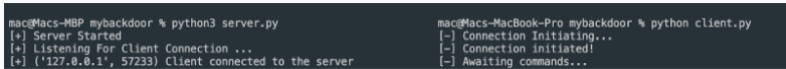
\includegraphics[height = 5 cm]{6.png}
\end{center}
Se va face corectura de rigoare și vom avea astfel:

\begin{center}
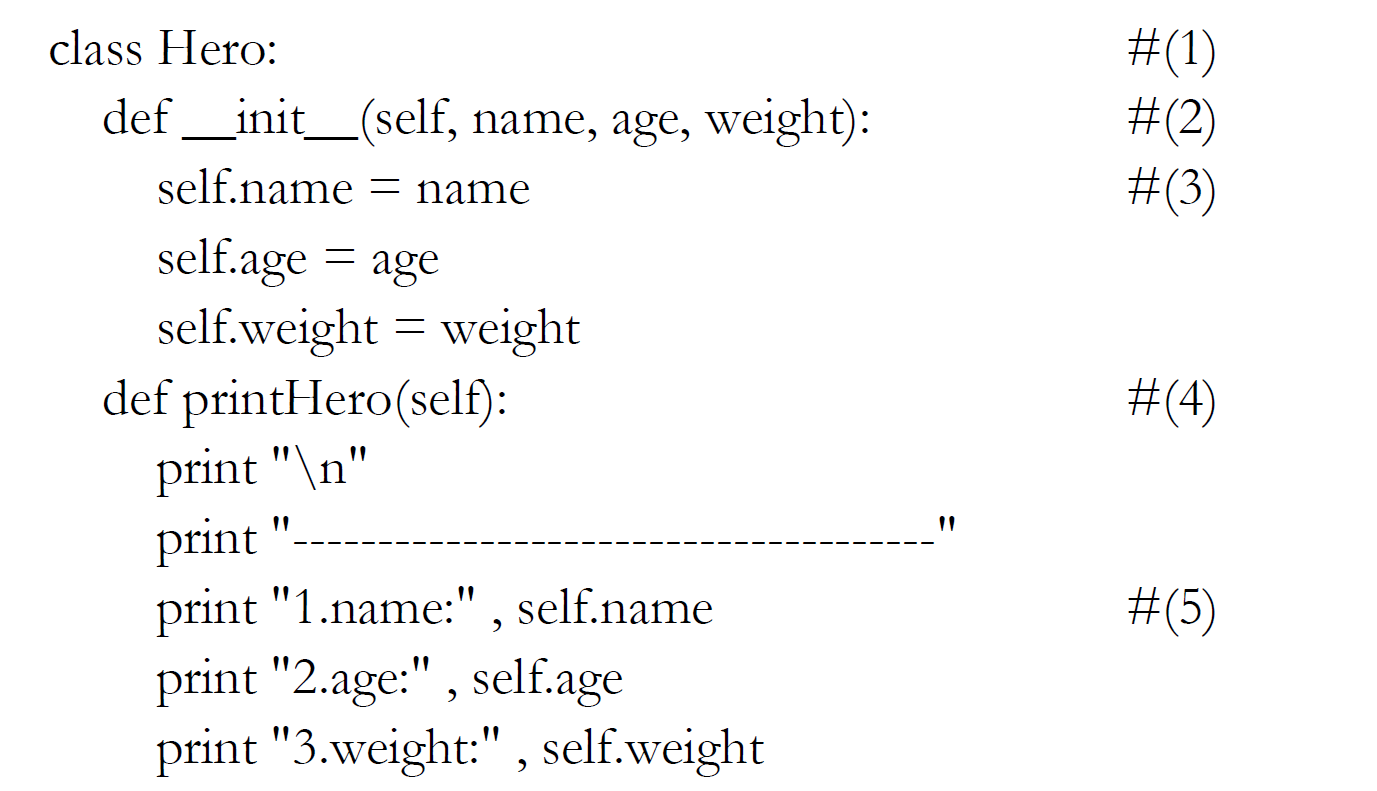
\includegraphics[height = 5 cm]{7.png}
\end{center}

\section{Bibliografie}

Python Hacking Essentials Paperback 2015 by Earnest Wish, \\
https://www.amazon.com/Python-Hacking-Essentials-Earnest-Wish/dp/1511797568


\end{document}
